\documentclass[a4paper,12pt]{article}
\usepackage{mathtools,amsfonts,amssymb,amsmath, bm,commath,multicol}
\usepackage{algorithmicx, tkz-graph, algorithm, fancyhdr, pgfplots}
\usepackage{fancyvrb}
\usepackage[backend=biber]{biblatex}
\addbibresource{review.bib}

\usepackage[noend]{algpseudocode}

\pagestyle{fancy}
\fancyhf{}
\rhead{30/5/2017 ::: Nandan Rao}
\lhead{Social and Economic Networks ::: Lit Review 1}
\rfoot{\thepage}

\begin{document}

\section*{Selfish Routing and Braess's Paradox}

We will use a 2006 paper from Tim Roughgarden \cite{selfish}, which acts as a review and strengthening of his earlier work (including that with Eva Tardos \cite{tardos} and that from his PhD dissertation \cite{thesis}), as a guide to dive into the background of these topics in a way that best supports our purposes. This work involves several important theorems bounding and proving the complexity of determining the Braess ratio among various networks. The main points regarding single-commodity graphs elucidated in this summary were also present in his earlier work \cite{designing}, and we point out the differences when they are noteworthy, however suffice to say it is most valuable to focus on this latest and most lucid paper.

One of the primary results will be that an upper bound of the price of anarchy in networks with linear latency functions is 4/3, but we will not focus on that here as that was well-covered in class. Another similar result is that the worst-case network with non-linear cost functions is provided, as well, by a Pigouvian network, and that the price of anarchy in that case is unbounded, but can be defined and bounded with any defined polynomial cost.

We will focus on the results regarding Braess's paradox. It is important to note that here we move from considering the difference between socially-efficient routing and nash equilibrium, and instead focus on network design and the cost difference between the worst-possible network versus that of its optimal subgraph, looking in both cases at the graphs during equilibrium. The price of anarchy will help us by providing some bounds for the Braess ratio, but is not of interest to us in and of itself.

In this paper, unlike in previous work, Roughgarden also gives due treatment to multicommodity networks, a network in which there are multiple sources and destinations, in contrast to previous work which focuses primarily on the single-commodity case.

\subsection*{The price of Braess's Paradox in single-commodity networks}

To understand this point we need to first define a Wardrop equilibrium, which simply says that given a certain flow $\textit{f}$, and cost function along a path $c_{\mathcal{P}}: \mathcal{P} \rightarrow \mathcal{R}^+$, the cost of every equilibrium path is a equal, and less than the cost along any non-equilibrium path:
%
$$
c_{\mathcal{P}}(\textit{f}) \leq c_{\widetilde{\mathcal{P}}}(\textit{f} )
$$
%
This is extended to the case of multicommodity by confirming that the above holds for every pair of possible paths in every commodity.

Now we can define Braess ratio, which as previously mentioned is what we are primarily interested in, rather than the price of anarchy. Namely the ratio between the Wardrop equilibrium of the full network, to that of its optimal subnetwork:
%
$$
\beta (G, r, c) = \max_{H \subset G} \frac{C(\textit{f})}{C(\textit{f}^H)}
$$
%
Given that the price of anarchy is
%
$$
\rho (G, r, c) = \frac{C(\textit{f})}{C(\textit{f}^*)}
$$
%
Any subnetwork H can be created as an optimal flow of G, therefore:
%
$$
C(\textit{f}^*) \geq C(\textit{f}^H)
$$
%
Which allows us to bound the Braess ratio, for single-commodity instances, by the price of anarchy:
%
$$
\beta (G, r, c) \leq \rho (G, r, c)
$$
%
This gives us the useful fact that the Braess ratio in a single-commodity network with linear cost functions is bounded by 4/3.

For nonlinear cost functions, where the price of anarchy skyrockets, however, this alone does not get us very far. By extending the Braess paradox, which consists of a graph of only 4 nodes, into a so-called Braess graph with a higher number of nodes, Roughgarden proves a lower-bound for the maximum Braess ratio of a given graph size, and then by exploiting the process of removing edges, proves an equivalent upper-bound on the maximum ratio as well. We treat each bound separately.

\subsubsection*{Lower bounding the Braess ratio}

This one is more straight forward, if we can define a Braess graph with the same ratio as the original, and extend this to any size n, we have proven that for any n there exists at least one graph with a Braess ratio of at least the size of this graph. The tricky part is therefore defining the extension of the Braess graph into any size n, which is beautifully done, and nicely shown in figure \ref{fig:kbraess}. 

\begin{figure}
  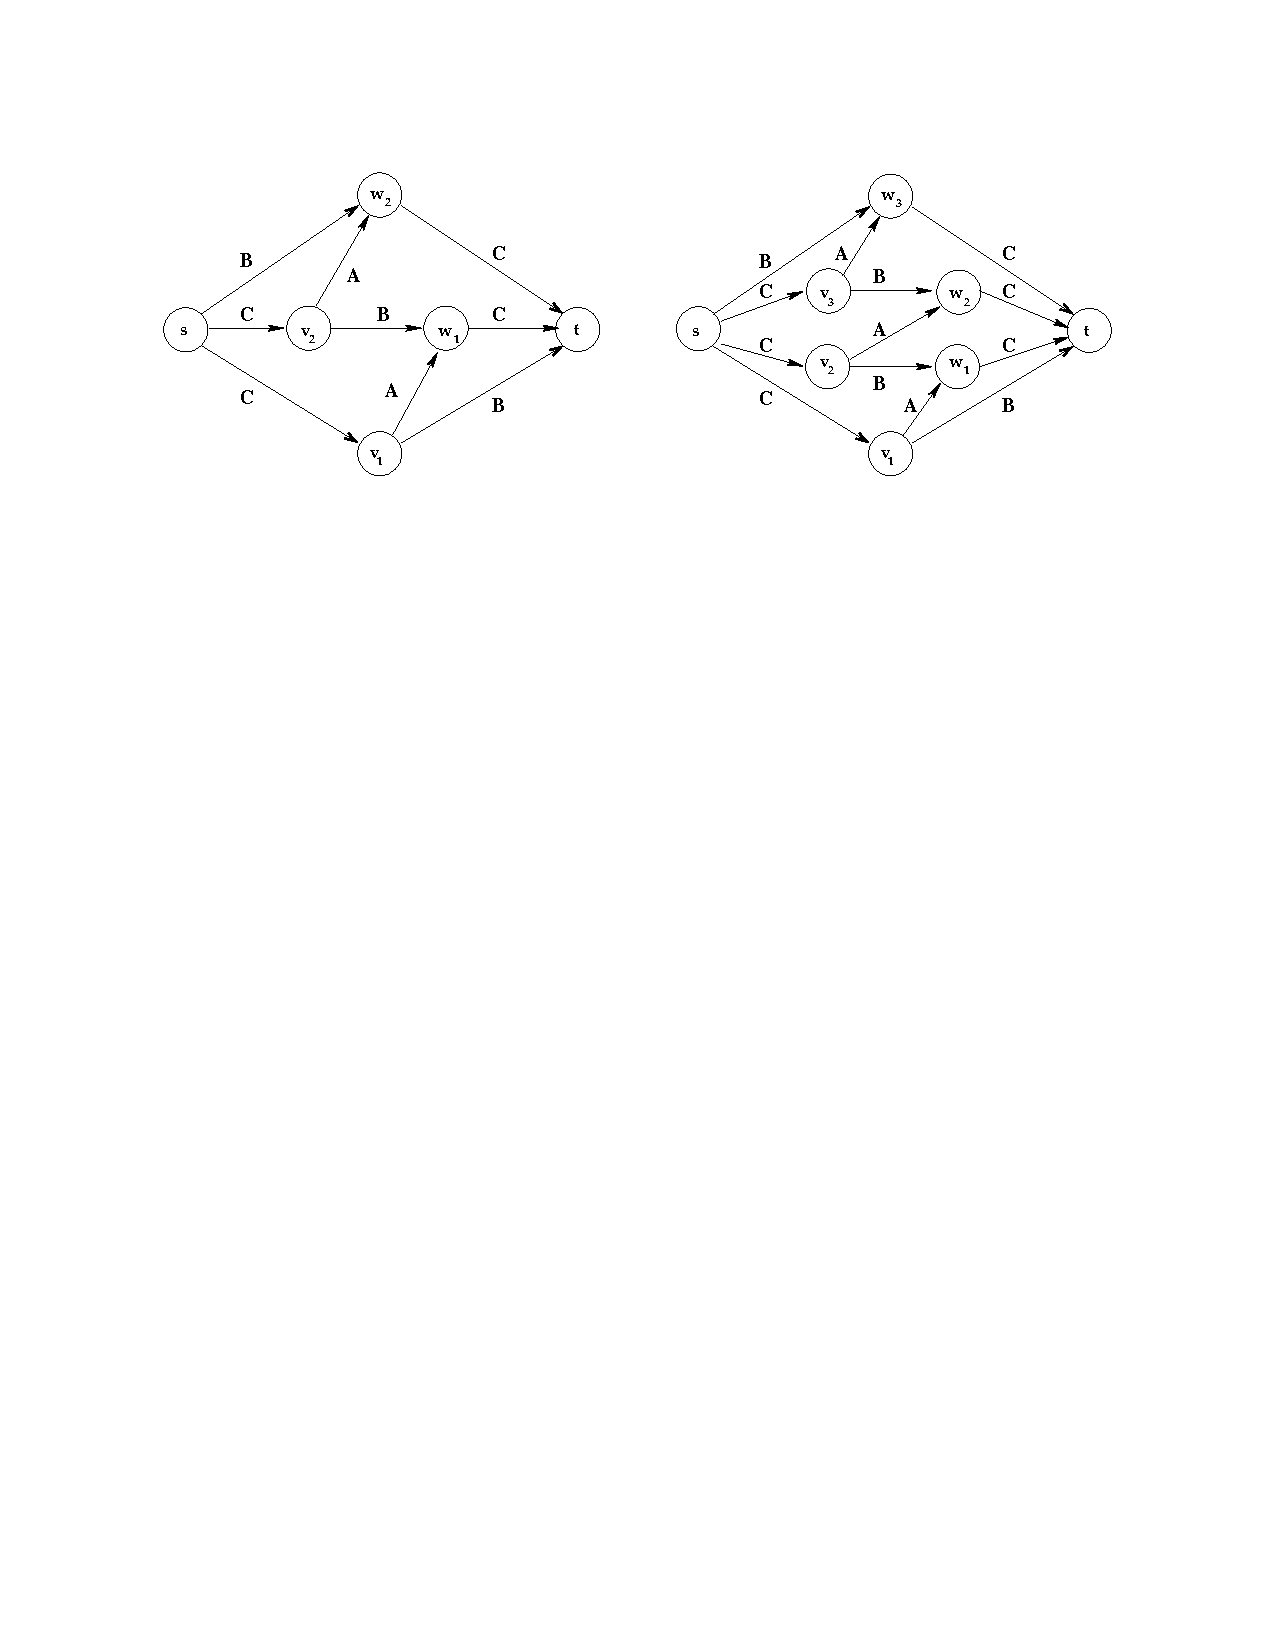
\includegraphics[width=\linewidth]{figures/optima.pdf}
  \caption{K Braess Graph}
  \label{fig:kbraess}
\end{figure}



\subsubsection*{Upper bounding the Braess ratio}

Interestingly, this is one of the proofs that has changed most markedly from Roughgarden's earlier paper (On the severity of Braess’s Paradox: Designing networks for selfish users is hard), and indeed this is both one of the most important parts of his work for our purposes, but also one of the most difficult to prove nicely.

I will provide an intuitive explanation without diving into the details, as I don't see any way to provide a formal treatment that is any more succinct than what he has written, in either case, as both are quite convoluted. The basic idea comes down to characterizing paths as Light or Heavy. A Light path is one which has more flow in the restricted subgraph then in the original, Heavy is a path which has less. Naturally, paths in which edges have been removed, will themselves have a flow of zero in the restricted graph, and are therefore Heavy.

The proof now consists of two parts: first, upper bound the potential gain from a Heavy path. Second, upper bound the number of such paths which can exist. The second part is the one that changes radically from one paper to the other, and consists of exploiting the conservancy of total input/output flow in subgraphs to prove that at most n/2 such heavy paths can exist.

The first part is easy to explain formally. Consider two paths, one heavy, and one light, that go from the source, s, to a given node, v. Consider a distance function, d, for the distance in the original graph and d* for the distance in the original graph. The distance to node v, d(v), must be equal along both paths (or the original graph isn't in equilibrium):
%
$$
d_H(v) = d_L(v)
$$
By definition of a Light path, the flow along the Light path has increased in the restricted subgraph, and given the non-decreasing nature of our cost functions:
$$
d_L(v) \leq d^*_L(v)
$$
%
Naturally, the distance to any node, $d^*(v)$, must be less than or equal to that of the end node, and therefore less than or equal to the total cost of the restricted subgraph:
%
$$
d_H(v) = d_L(v) \leq d^*_L(v) \leq d^*(t) = C(\textit{f}^H)
$$
%
This leads to the following upper-bound on the maximum Braess ratio:
%
$$
\beta (G, r, c) \leq \frac{n}{2} \beta(H, r, c)
$$
%

\subsection*{Multicommodity networks}
Roughgarden's paper \cite{selfish} contains information about multicommodity networks primarily as a review of Lin's 2005 work \cite{fibonacci}, which we will consider directly.

Lin's paper consists of two parts, proving a lower-bound on the maximum price of anarchy in multicommodity networks through an invention of their own crafted, so-called fibonacci network, and then a proving a close upper-bound through a linear program.

\subsubsection*{Lower bound}

This is an extremely inelegant example. It involves a designed network in which paths alternate between fixed and flexible costs, orthogonal paths between commodities, with the flexible costs increasing as one gets closer to ones destination, and paths between that trap the poor particles in a diabolical this-will-only-ever-get-worse-for-you torture chamber of a path. I provide a picture in figure \ref{fig:toture}.

\begin{figure}
  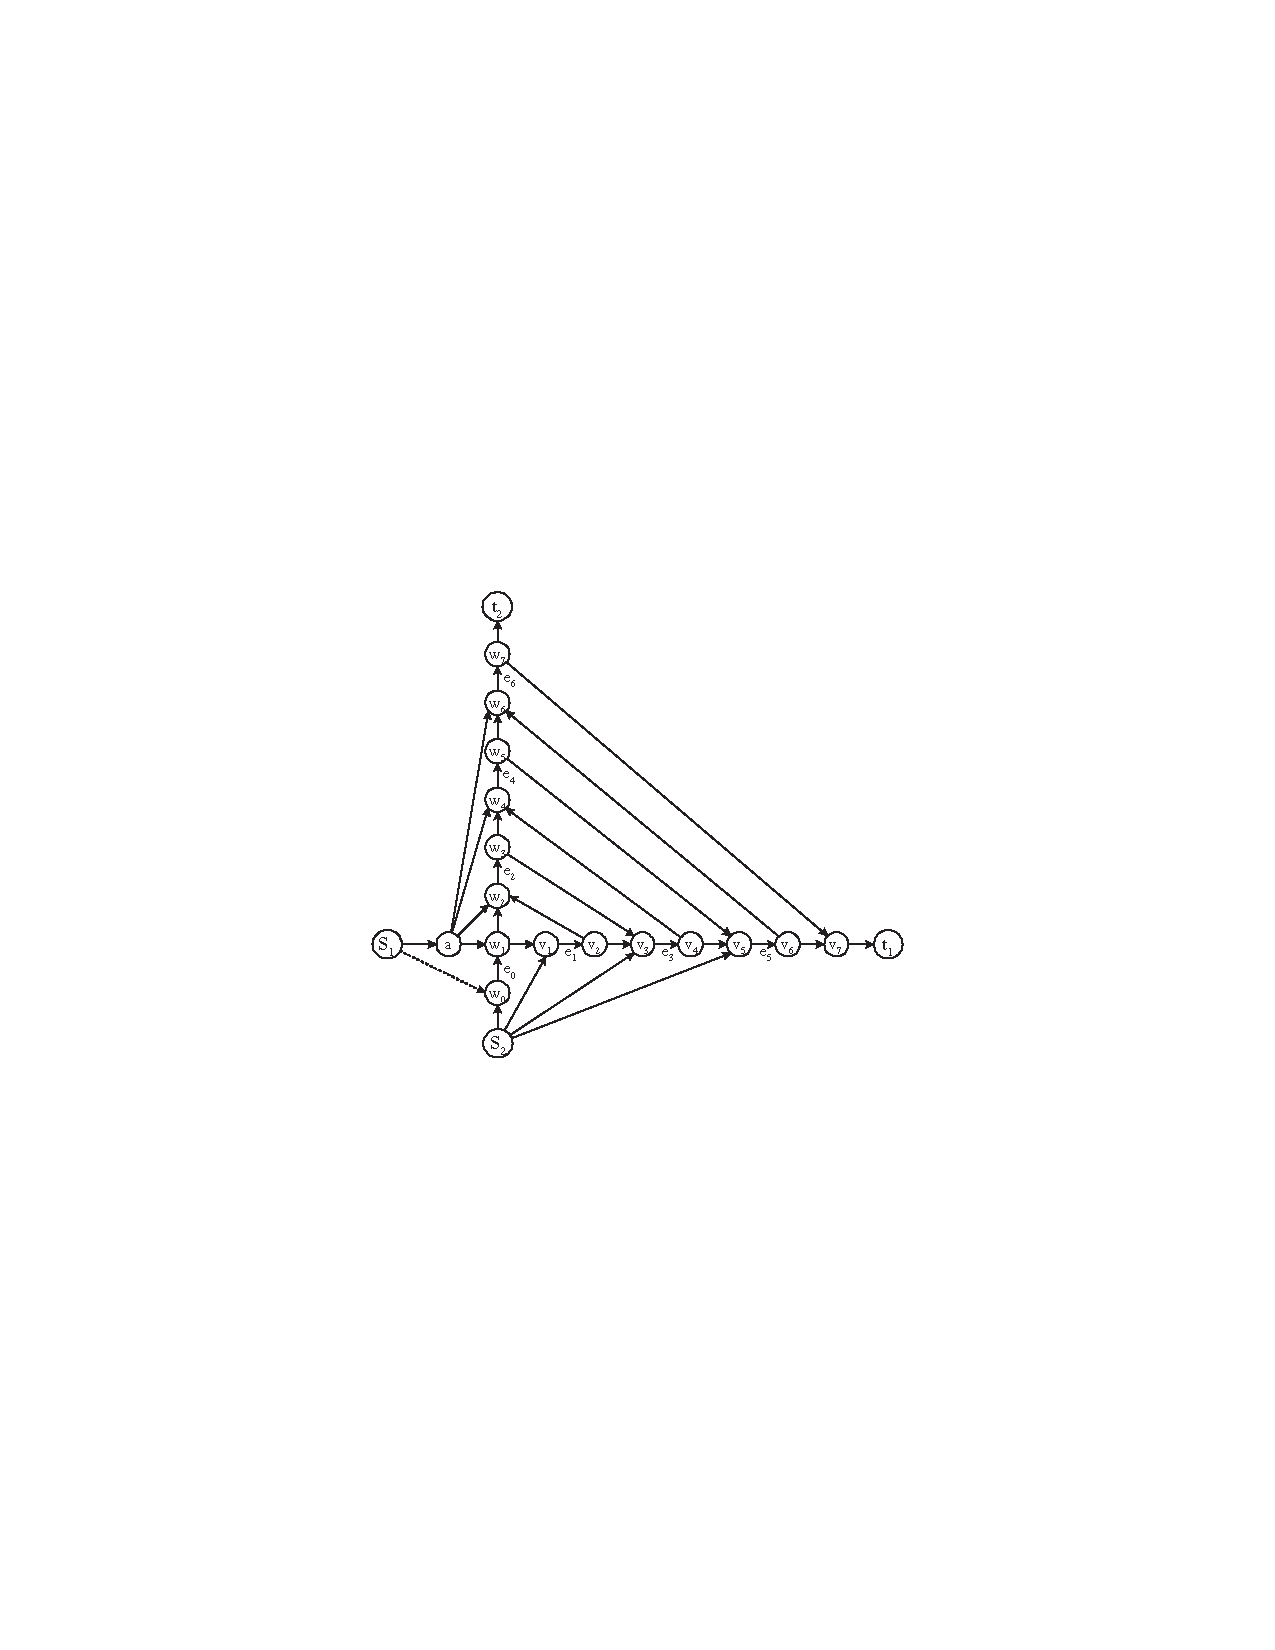
\includegraphics[width=\linewidth]{figures/cropped_mcbp.pdf}
  \caption{Torture Chamber}
  \label{fig:torture}
\end{figure}



\subsubsection*{Upper bound}

There are two upper bounds proven here, the first a crude one that comes directly from the formulation of the problem, the second comes from using the first in a series of linear programming excersizes, and results in the following two bounds: 
%
$$
\rho (G, r, c) = 2^{O(M log n)}
$$
%
Which holds for graphs with any number of commodities, and when the number is small, this can be treated as a constant to prove the following bounds: 
%
$$
\rho (G, r, c) = 2^{O(kn)}
$$
%
\subsection*{Detecting Braess's paradox}
Here we examine the single-commodity and multicommodity separately, the first which was considered by Roughgarden \cite{designing}, the second by Lin \cite{fibonacci}. 

\subsubsection*{Single-commodity design}

The single-commodity proof piggy-backs on a proof of complexity for solving the problem of 2 Directed Disjoint Paths \cite{fortune}. The basic concept is, given two nodes $s_1, s_2$, and two others $t_1, t_2$, can we find vertex-disjoint $s_i-t_i$ paths in polynomial time? By adding a single source that leads to the s nodes, and a single sink that recieves from the t nodes, Roughgarden shows that if it were possible to discover a better network design than the trivial algorithm in polynomial time, that could be used to solve the 2DDP problem, which would then not be NP-hard. See figure \ref{fig:2DDP}.
 
\begin{figure}
  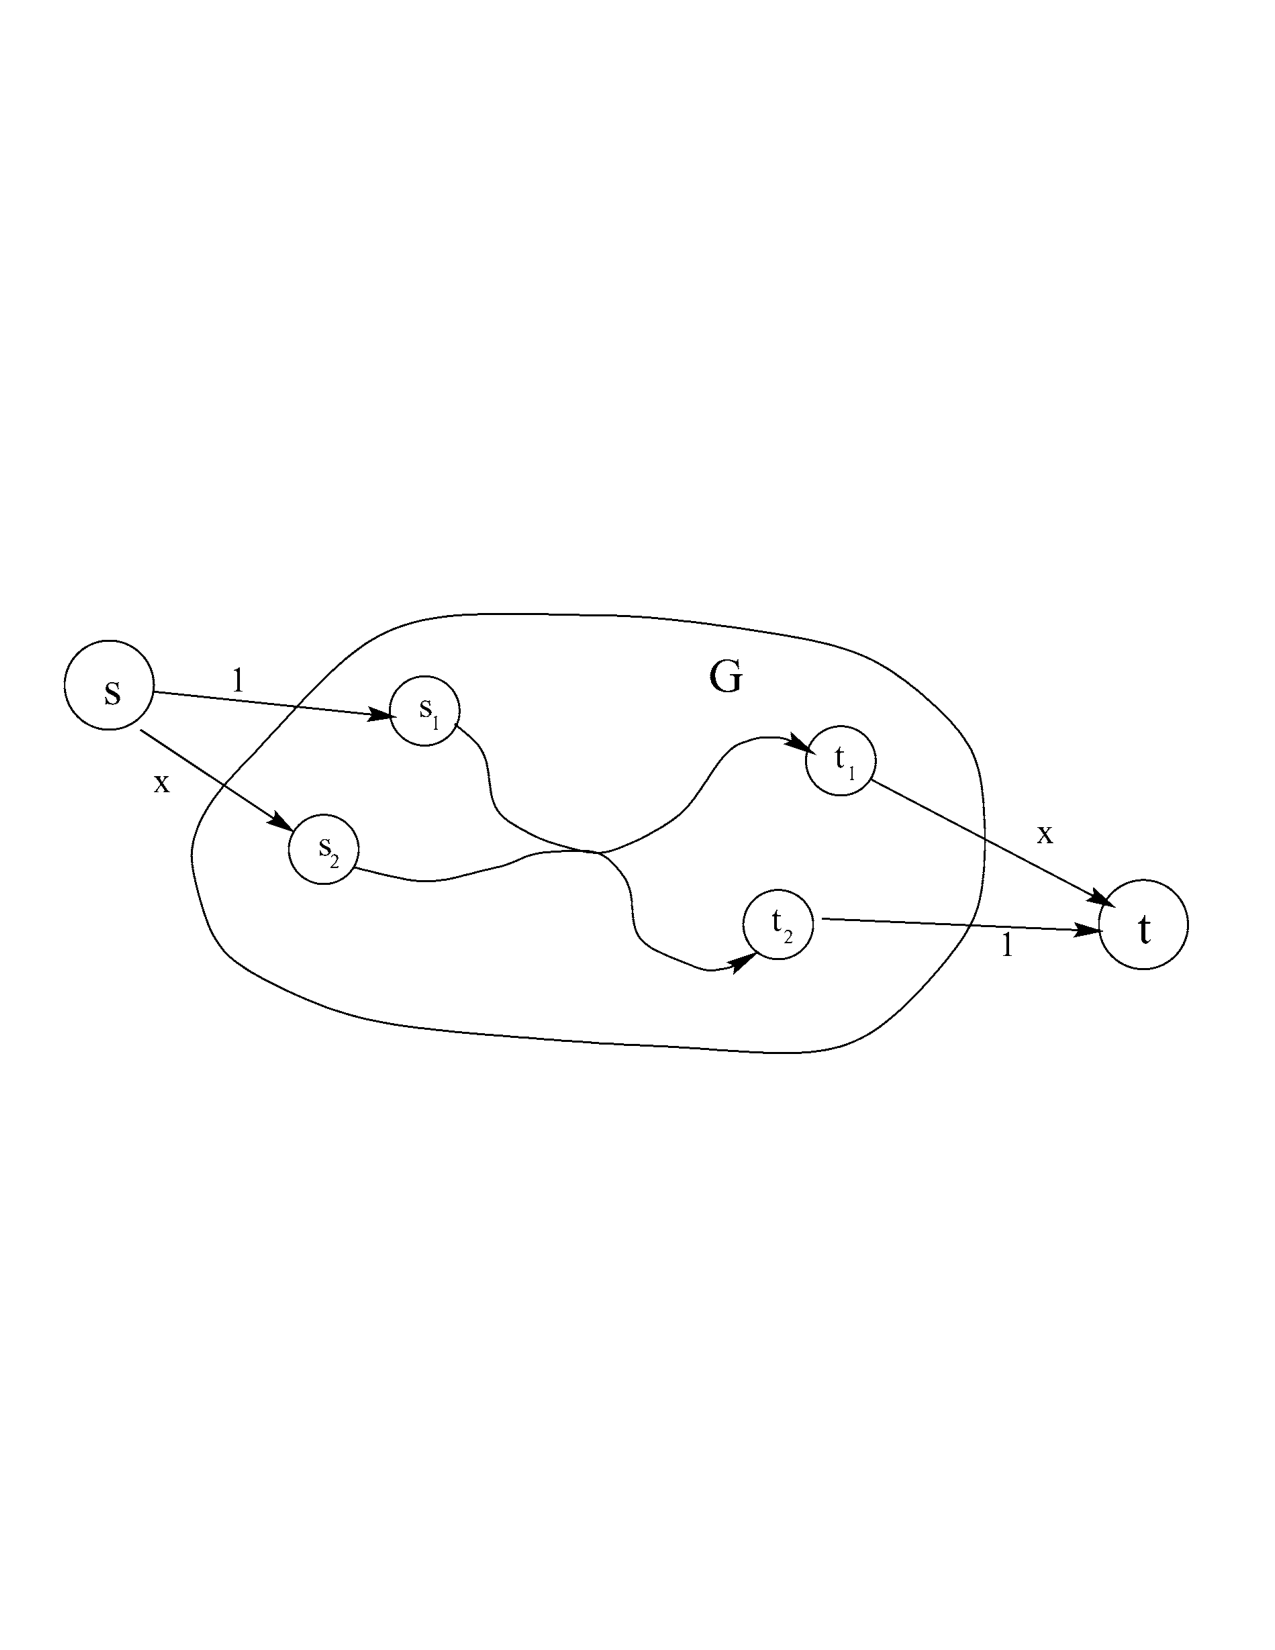
\includegraphics[width=\linewidth]{figures/cropped_proof-of-4-3-bounds.pdf}
  \caption{Solving 2DDP with Network Design}
  \label{fig:2DDP}
\end{figure}


\subsubsection*{Single-commodity design}
The multicommodity version is in approach very similar to that of the single-commodity one, referring to the known NP-complete problem Partition, and showing that if the multicommodity network design problem were solvable in polynomial time, so would Partition. 


\printbibliography
\end{document}